\mode*

\begin{frame}{Problématique du cours}
    \begin{shadequote}{Maurice Herlihy \& Nir Shavit}
    For many of the applications you may wish to parallelize, you will find that there are significant parts that can easily be determined
    as executable in parallel because they do not require any form of coordination or communication. However, (...)
    \alert{there is no cookbook recipe for identifying these parts}. This is where the application designer needs to use
    his or her accumulated understanding of the algorithm being parallelized. Luckily, in many cases it is obvious how to find such parts.
    
    \vspace{4mm}
    \alert{The more substantial problem} (...)
    \alert{is how to deal with the remaining parts of the program.} As noted earlier, these are the parts that cannot be easily parallelized
    because the program must access shared data and requires interprocess coordination and communication in an essential way.
    \end{shadequote}
\end{frame}

\begin{frame}{Du parallélisme à la concurrence}
\begin{center}
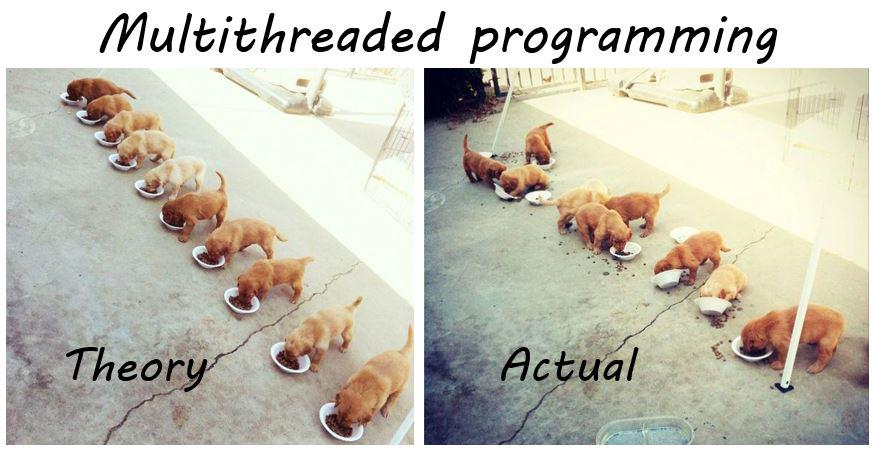
\includegraphics[width=\textwidth]{pupies}
\end{center}
\end{frame}


%%%%%%%%%%%%%%%%%%%%%%%%%%%%%%%%%%%%%%%%%%%%%%%%%%%%%%%%%%%%%%%%%%%%%%%%%

\begin{frame}{Parallélisme versus concurrence}
  \vFill
  \begin{block}{Principale difficulté}
    \begin{description}
    \item[Parallélisme :] Identifier les tâches indépendantes
    \item[Concurrence :] Gérer l'incertitude
    \end{description}
    \begin{shadequote}{Leslie Lamport}
    A distributed system is one in which the failure of a computer you didn't even know existed can render your own computer unusable.
    \end{shadequote}
  \end{block}
  \vFill
  \uncover<2->{
  \begin{block}{Contexte d'exécution}
    \begin{description}
    \item[Parallélisme :] Choisi en fonction du problème à résoudre
    \item[Concurrence :] Imposé \textit{a priori} par le problème
    \end{description}
  \end{block}
  }
  \vFill
  \uncover<3->{
  \begin{block}{Passage à l'échelle}
    \begin{minipage}{.5\textwidth}
      \begin{description}
      \item[Parallélisme :] $S_p(n) = \Omega(n)$
      \end{description}
    \end{minipage}\begin{minipage}{.45\textwidth}
      \begin{description}
      \item[Concurrence :] $S_c(n) = \Omega(1)$
      \end{description}
    \end{minipage}
  \end{block}
  }
  \vFill
  \begin{citing}
  \item[R15] Michel Raynal. \textit{Parallel Computing vs. Distributed Computing: A Great Confusion? (Position Paper).} Euro-Par Workshops (2015).
  \end{citing}
\end{frame}

\begin{frame}{Point vocabulaire}
  \begin{tabular}{ccc}
    &Une seule unité d'exécution & Plusieurs unités d'exécution
    \\
    
\begin{tikzpicture}
        \draw[white] (0, 0) rectangle (2,3);
        \draw (1, 1.75) node{Problème};
        \draw (1, 1.25) node{Séquentiel};
    \end{tikzpicture}
&
    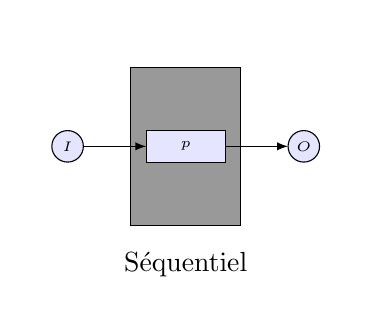
\begin{tikzpicture}

        \draw[white] (-0.5, -0.3) rectangle (3.5,3);
        \draw (1.5, 0) node{Séquentiel};

        \draw[fill=black!40] (0.8, 0.5) rectangle (2.2,2.5);
        \draw[fill=blue!10] (1.5, 1.5) +(-0.5, -.2) rectangle +(0.5, .2) +(0,0) node{\tiny $p$};

        \draw[-latex] (0.2, 1.5) -- (1,1.5);
        \draw[-latex] (2, 1.5) -- (2.8,1.5);

        \draw[fill=blue!10] (0, 1.5) circle (2mm) node{\tiny $I$};
        \draw[fill=blue!10] (3, 1.5) circle (2mm) node{\tiny $O$};
      \end{tikzpicture}
&
      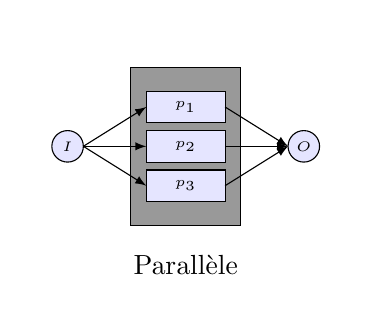
\begin{tikzpicture}
        \draw[white] (-0.5, -0.3) rectangle (3.5,3);
        \draw (1.5, 0) node{Parallèle};

        \draw[fill=black!40] (0.8, 0.5) rectangle (2.2,2.5);
        \draw[fill=blue!10] (1.5, 2) +(-0.5, -.2) rectangle +(0.5, .2)   +(0,0) node{\tiny $p_1$};
        \draw[fill=blue!10] (1.5, 1.5) +(-0.5, -.2) rectangle +(0.5, .2) +(0,0) node{\tiny $p_2$};
        \draw[fill=blue!10] (1.5, 1) +(-0.5, -.2) rectangle +(0.5, .2)   +(0,0) node{\tiny $p_3$};

        \draw[-latex] (0.2, 1.5) -- (1,2);
        \draw[-latex] (0.2, 1.5) -- (1,1.5);
        \draw[-latex] (0.2, 1.5) -- (1,1);

        \draw[-latex] (2, 2)   -- (2.8,1.5);
        \draw[-latex] (2, 1.5) -- (2.8,1.5);
        \draw[-latex] (2, 1)   -- (2.8,1.5);

        \draw[fill=blue!10] (0, 1.5) circle (2mm) node{\tiny $I$};
        \draw[fill=blue!10] (3, 1.5) circle (2mm) node{\tiny $O$};
      \end{tikzpicture}
    \\
    
\begin{tikzpicture}
        \draw[white] (0, 0) rectangle (2,3);
        \draw (1, 1.75) node{Problème};
        \draw (1, 1.35) node{de};
        \draw (1, 0.95) node{concurrence};
    \end{tikzpicture}
    &
      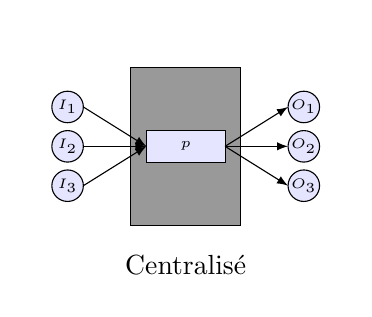
\begin{tikzpicture}
        \draw[white] (-0.5, -0.3) rectangle (3.5,3);
        \draw (1.5, 0) node{Centralisé};

        \draw[fill=black!40] (0.8, 0.5) rectangle (2.2,2.5);
        \draw[fill=blue!10] (1.5, 1.5) +(-0.5, -.2) rectangle +(0.5, .2) +(0,0) node{\tiny $p$};

        \draw[-latex] (0.2, 2) -- (1,1.5);
        \draw[-latex] (0.2, 1.5) -- (1,1.5);
        \draw[-latex] (0.2, 1) -- (1,1.5);

        \draw[-latex] (2, 1.5) -- (2.8,2);
        \draw[-latex] (2, 1.5) -- (2.8,1.5);
        \draw[-latex] (2, 1.5) -- (2.8,1);

        \draw[fill=blue!10] (0, 2) circle (2mm)   node{\tiny $I_1$};
        \draw[fill=blue!10] (0, 1.5) circle (2mm) node{\tiny $I_2$};
        \draw[fill=blue!10] (0, 1) circle (2mm)   node{\tiny $I_3$};

        \draw[fill=blue!10] (3, 2) circle (2mm)   node{\tiny $O_1$};
        \draw[fill=blue!10] (3, 1.5) circle (2mm) node{\tiny $O_2$};
        \draw[fill=blue!10] (3, 1) circle (2mm)   node{\tiny $O_3$};
      \end{tikzpicture}
      &
      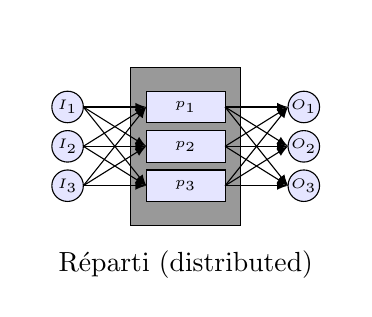
\begin{tikzpicture}
        \draw[white] (-0.5, -0.3) rectangle (3.5,3);
        \draw (1.5, 0) node{Réparti (distributed)};

        \draw[fill=black!40] (0.8, 0.5) rectangle (2.2,2.5);
        \draw[fill=blue!10] (1.5, 2) +(-0.5, -.2) rectangle +(0.5, .2)   +(0,0) node{\tiny $p_1$};
        \draw[fill=blue!10] (1.5, 1.5) +(-0.5, -.2) rectangle +(0.5, .2) +(0,0) node{\tiny $p_2$};
        \draw[fill=blue!10] (1.5, 1) +(-0.5, -.2) rectangle +(0.5, .2)   +(0,0) node{\tiny $p_3$};

        \draw[-latex] (0.2, 2) -- (1,2);
        \draw[-latex] (0.2, 2) -- (1,1.5);
        \draw[-latex] (0.2, 2) -- (1,1);

        \draw[-latex] (0.2, 1.5) -- (1,2);
        \draw[-latex] (0.2, 1.5) -- (1,1.5);
        \draw[-latex] (0.2, 1.5) -- (1,1);
                         
        \draw[-latex] (0.2, 1) -- (1,2);
        \draw[-latex] (0.2, 1) -- (1,1.5);
        \draw[-latex] (0.2, 1) -- (1,1);

        \draw[-latex] (2, 2)   -- (2.8,2);
        \draw[-latex] (2, 2)   -- (2.8,1.5);
        \draw[-latex] (2, 2)   -- (2.8,1);
                                    
        \draw[-latex] (2, 1.5) -- (2.8,2);
        \draw[-latex] (2, 1.5) -- (2.8,1.5);
        \draw[-latex] (2, 1.5) -- (2.8,1);
                                    
        \draw[-latex] (2, 1)   -- (2.8,2);
        \draw[-latex] (2, 1)   -- (2.8,1.5);
        \draw[-latex] (2, 1)   -- (2.8,1);

        \draw[fill=blue!10] (0, 2) circle (2mm)   node{\tiny $I_1$};
        \draw[fill=blue!10] (0, 1.5) circle (2mm) node{\tiny $I_2$};
        \draw[fill=blue!10] (0, 1) circle (2mm)   node{\tiny $I_3$};

        \draw[fill=blue!10] (3, 2) circle (2mm)   node{\tiny $O_1$};
        \draw[fill=blue!10] (3, 1.5) circle (2mm) node{\tiny $O_2$};
        \draw[fill=blue!10] (3, 1) circle (2mm)   node{\tiny $O_3$};
      \end{tikzpicture}
      \end{tabular}
\end{frame}

\begin{frame}{Exercice}

  \begin{alertblock}{Problème de parallélisme ou de concurrence ?}
    \begin{enumerate} 
    \item Éviter les collisions sur la route.
    \item Optimiser la vitesse de production d'une usine (Fordisme).
    \item Élire le président de la république.
    \item Massively multiplayer online role-playing game.
    \item Prévoir la météo.
    \item Les projets semestriels en groupe.
    \item Un orchestre symphonique.
    \end{enumerate} 
  \end{alertblock}
\end{frame}

\mode<all>


